\begin{figure}[tbp]
\centering
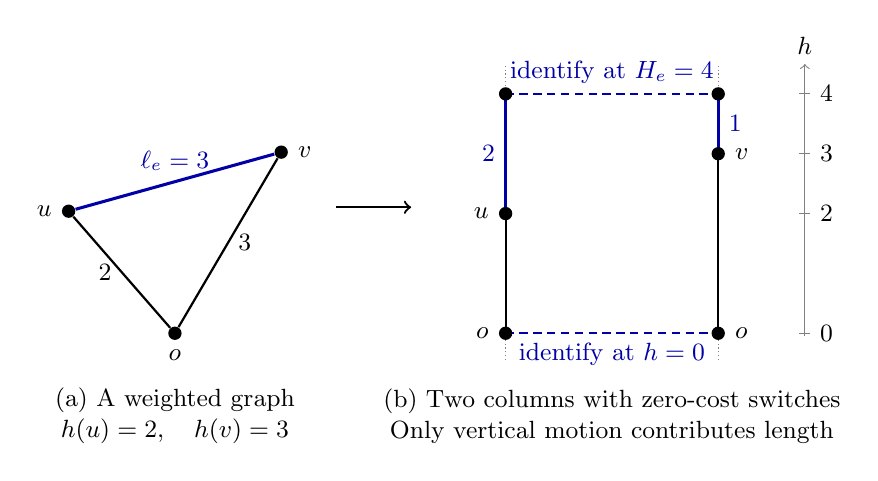
\begin{tikzpicture}[x=1cm,y=1cm,font=\small,
  vertex/.style={circle,fill=black,inner sep=1.7pt},
  twig/.style={blue!65!black,line width=1.1pt},
  identify/.style={blue!65!black,densely dashed,line width=.8pt}]
  \node[vertex,label=below:$o$] (o) at (0,0) {};
  \node[vertex,label=left:$u$] (u) at (-1.35,1.55) {};
  \node[vertex,label=right:$v$] (v) at (1.35,2.3) {};
  \draw[thick] (o)--node[left] {$2$} (u);
  \draw[thick] (o)--node[right] {$3$} (v);
  \draw[twig] (u)--node[above] {$\ell_e=3$} (v);
  \node[align=center] at (0,-1.05) {(a) A weighted graph\\$h(u)=2,\quad h(v)=3$};

  \draw[->,thick] (2.05,1.6)--(3,1.6);

  \begin{scope}[shift={(4.2,0)},y=.76cm]
    \draw[gray,densely dotted] (0,-.45)--(0,0);
    \draw[gray,densely dotted] (2.7,-.45)--(2.7,0);
    \draw[thick] (0,0)--(0,2);
    \draw[thick] (2.7,0)--(2.7,3);
    \draw[twig] (0,2)--node[left] {$2$} (0,4);
    \draw[twig] (2.7,3)--node[right] {$1$} (2.7,4);
    \draw[gray,densely dotted] (0,4)--(0,4.5);
    \draw[gray,densely dotted] (2.7,4)--(2.7,4.5);
    \draw[identify] (0,0)--node[below] {identify at $h=0$} (2.7,0);
    \draw[identify] (0,4)--node[above] {identify at $H_e=4$} (2.7,4);
    \node[vertex,label=left:$o$] at (0,0) {};
    \node[vertex,label=right:$o$] at (2.7,0) {};
    \node[vertex,label=left:$u$] at (0,2) {};
    \node[vertex,label=right:$v$] at (2.7,3) {};
    \node[vertex] at (0,4) {};
    \node[vertex] at (2.7,4) {};
    \draw[->,gray] (3.8,-.05)--(3.8,4.5) node[above,black] {$h$};
    \foreach \h in {0,2,3,4} {
      \draw[gray] (3.73,\h)--(3.87,\h) node[right,black] {$\h$};
    }
  \end{scope}
  \node[align=center] at (5.55,-1.05) {(b) Two columns with zero-cost switches\\Only vertical motion contributes length};
\end{tikzpicture}
\caption{An exact example of Proposition~\ref{geo:realization}.
The black edges form a shortest-path tree rooted at $o$.
The non-tree edge is replaced by two ascending twigs of lengths
$(\ell_e+h(v)-h(u))/2=2$ and $(\ell_e+h(u)-h(v))/2=1$.
Their tips have the same height $H_e=4$ and are identified.
Dashed horizontal segments denote identifications, not extra edges;
the dotted vertical tails do not shorten original distances.}
\label{fig:column-realization}
\end{figure}
